\documentclass[aspectratio=43,10pt]{beamer}
\usetheme{default}
\usecolortheme{default}
\setbeamertemplate{navigation symbols}{}
\setbeamertemplate{footline}[frame number]
\setbeamertemplate{itemize items}[circle]
\usepackage[T1]{fontenc}
\usepackage{lmodern}
\usepackage{amsmath,amssymb,booktabs,graphicx,xcolor,listings}
\setbeamertemplate{navigation symbols}{}
\setbeamertemplate{footline}[frame number]
\definecolor{aggiemaroon}{RGB}{80,0,0}
\setbeamertemplate{itemize items}[circle]
\definecolor{oce}{HTML}{126A8C}
\definecolor{ice}{HTML}{E7F3F7}
\definecolor{ink}{HTML}{18303A}
\setbeamercolor{frametitle}{fg=aggiemaroon}
\setbeamercolor{title}{fg=aggiemaroon}
\setbeamercolor{structure}{fg=aggiemaroon}

\lstdefinelanguage{Rcode}{keywords={library,data,table,dim,str,glimpse,count,group_by,summarise,mean,filter,pull,na.omit,length,qnorm,sqrt,rnorm,ggplot,aes,geom_density,geom_point,geom_smooth,mutate,select,drop_na,stan_glm,normal,exponential,update,summary,prior_summary,posterior_interval,predictive_interval,posterior_epred,posterior_predict,pp_check,plot,brm,prior,as.matrix,colnames,set.seed,sample,seq_len,nrow,crossing,row_number,quantile,as.vector,factor,lapply,do.call,head,hist},sensitive=true,morecomment=[l]{\#},morestring=[b]"}
\lstset{language=Rcode,basicstyle=\ttfamily\small,keywordstyle=\color{oce}\bfseries,commentstyle=\color{gray},stringstyle=\color{orange!70!black},showstringspaces=false,breaklines=true,columns=fullflexible,keepspaces=true,frame=single,rulecolor=\color{black!15},backgroundcolor=\color{ice!23},aboveskip=3pt,belowskip=3pt}
\newcommand{\take}[1]{\begin{block}{}#1\end{block}}
\newcommand{\img}[2][0.82]{\begin{center}\includegraphics[width=#1\linewidth,height=0.66\textheight,keepaspectratio]{assets/#2}\end{center}}

\title{Decision and Risk Analysis}
\subtitle{Lecture 10: \textbf{Bayesian Penguins}}
\author{}
\date{\color{aggiemaroon}{DAEN 427 / ISEN 427 / ISEN 627 - Fall 2026\\
      \textbf{Alexander Abuabara}}}
\titlegraphic{\vfill 
\includegraphics[height=1.2cm]{TAMU_logo.png} \vspace{4ex} \par}


\begin{document}
\begin{frame}[plain]
\titlepage
\vspace{-0.7cm}
\begin{center}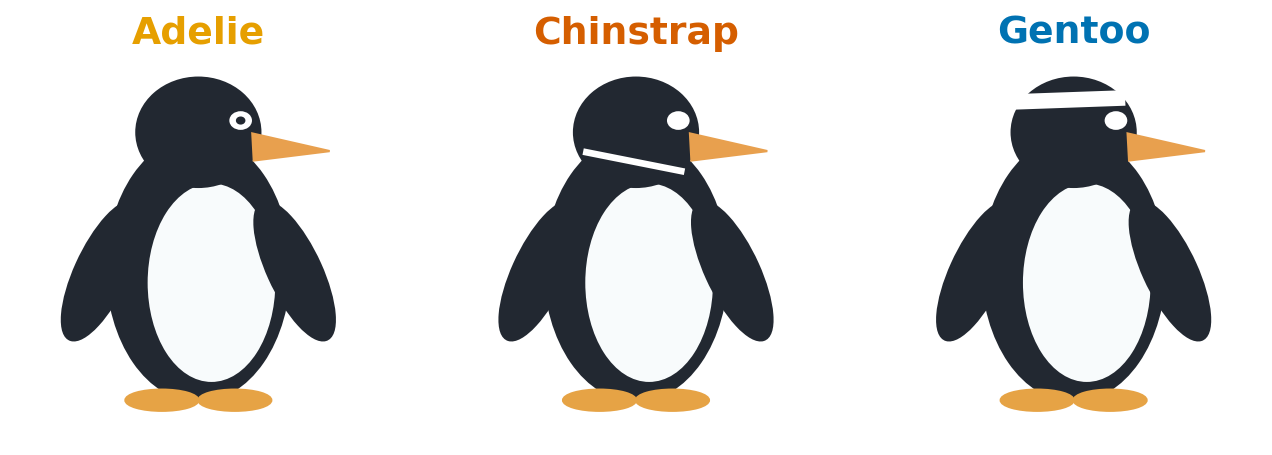
\includegraphics[width=.76\linewidth,height=2.2cm,keepaspectratio]{assets/species.png}\end{center}
\end{frame}

\begin{frame}{Learning goals: the penguin mission}
\begin{enumerate}\item Explore a real.
\item Update beliefs using a conjugate Normal model.
\item Fit Bayesian regression in \texttt{rstanarm} (and \texttt{brms}).
\item Separate \emph{prior}, \emph{posterior}, and \emph{predictive} distributions.
\item Check models, forecast a new penguin, and choose an action.
\item Get started on hierarchical models.
\end{enumerate}
%\take{Prediction answers ``what might happen?'' Decision analysis answers ``what should we do?''}
\end{frame}

\begin{frame}{Meet our colleagues}
\img[.95]{species.png}
\small The sample records \textbf{Adelie, Chinstrap, and Gentoo} penguins from the Palmer Archipelago.
\tiny Data: Palmer penguins, Gorman et al. (2014), via \texttt{bayesrules}/\texttt{palmerpenguins}.
\end{frame}

\begin{frame}[fragile]{1. Load packages and the dataset}
\begin{lstlisting}
library(tidyverse)  # dplyr, ggplot2, tidyr, ...
library(bayesrules) # teaching data and conjugate helpers
library(rstanarm)  # Bayesian regression with Stan
library(bayesplot) # Bayesian diagnostic plotting

data("penguins_bayes", package = "bayesrules")
penguins <- penguins_bayes
\end{lstlisting}
\begin{itemize}\item \texttt{library()} attaches functions; \texttt{data()} loads a packaged object.
\item \texttt{<-} assigns an R object. \texttt{penguins} is a convenient copy/reference.
\item 344 rows; 9 columns, including \texttt{above\_average\_weight}.
\end{itemize}
%\take{Packages provide tools; the data object provides observations.}
\end{frame}

\begin{frame}[fragile]{2. Inspect before modeling}
\begin{lstlisting}
table(penguins$year, penguins$species)
dim(penguins)          # row count and column count
str(penguins)          # base R structure
glimpse(penguins_bayes) # tidyverse structure
penguins %>% count(species)
\end{lstlisting}
\begin{itemize}\item \texttt{\$} extracts a column; \texttt{table()} cross-tabulates two categorical columns.
\item \texttt{\%>\%} pipes an object into the next function.
\item \texttt{count(species)} groups and counts the three species.
\end{itemize}
\img[.6]{counts.png}
\end{frame}

\begin{frame}[fragile]{3. Summaries by species}
\begin{lstlisting}
penguins %>%
  group_by(species) %>%
  summarise(
    n = n(),
    flipper_mean = mean(flipper_length_mm, na.rm=TRUE),
    bill_mean = mean(bill_length_mm, na.rm=TRUE),
    mass_mean = mean(body_mass_g, na.rm=TRUE),
    .groups = "drop"
  )
\end{lstlisting}
\small \texttt{group\_by()} defines the comparison groups; \texttt{summarise()} collapses each group to one row; \texttt{n()} counts rows; \texttt{na.rm=TRUE} prevents missing observations from making the mean missing; \texttt{.groups="drop"} returns an ungrouped result.\par
\take{One row per species, but each mean uses only nonmissing values in its variable.}
\end{frame}

\begin{frame}{Explore flippers: one species or three stories?}
\img[.8]{flippers.png}
\small If species have different typical flipper lengths, what might a single pooled regression miss?\par
\take{A good model starts with plots, not just a formula.}
\end{frame}

\begin{frame}{Bayes in one sentence}
\[\underbrace{p(\theta\mid y)}_{\text{posterior}}
\propto \underbrace{p(y\mid\theta)}_{\text{likelihood}}
\underbrace{p(\theta)}_{\text{prior}}\]
\begin{itemize}\item \(\theta\): unknown parameter; \(y\): observed measurements.
\item \textbf{Prior}: plausible parameter values before these observations.
\item \textbf{Likelihood}: which parameter values explain the data.
\item \textbf{Posterior}: updated parameter uncertainty after observing data.
\end{itemize}
\take{Bayesian inference produces a distribution, not only a best estimate.}
\end{frame}

\begin{frame}[fragile]{4. Encode a conjugate prior and likelihood}
\begin{lstlisting}
mu0 <- 190
prior_sd <- 10
sigma_known <- 7
\end{lstlisting}
\[\mu\sim N(190,10^2),\qquad y_i\mid\mu\sim N(\mu,7^2)\]
\vspace{-3ex}
\begin{itemize}\item \(\mu\): unknown average Adelie flipper length (mm).
\item \texttt{mu0}: prior mean; \texttt{prior\_sd}: prior uncertainty.
\item \texttt{sigma\_known}: \emph{assumed known} measurement/population spread.
\end{itemize}
\small This known-\(\sigma\) assumption makes the posterior analytically tractable, but should be justified or relaxed in real work.
\end{frame}

\begin{frame}[fragile]{5. Select observed Adelie measurements}
\begin{lstlisting}
y <- na.omit(penguins$flipper_length_mm[
  penguins$species == "Adelie"
])
n <- length(y)
y_bar <- mean(y)
\end{lstlisting}
\small Brackets \texttt{[condition]} select only matching rows; \texttt{na.omit()} excludes missing lengths; \texttt{length()} gives sample size; \texttt{mean()} computes \(\bar y\).\par
\begin{lstlisting}
# Equivalent tidyverse pipeline:
y <- penguins %>% filter(species == "Adelie") %>%
  pull(flipper_length_mm) %>% na.omit() %>% as.numeric()
\end{lstlisting}
\vspace{-3ex}
\take{In these records, \(n=151\) nonmissing Adelie flipper lengths, \(\bar y\approx189.95\) mm.}
\end{frame}

\begin{frame}{6. Derive the Normal--Normal posterior}
\[\sigma_{\mathrm{post}}^2=\left(\frac1{\tau_0^2}+\frac n{\sigma^2}\right)^{-1}\]
\[\mu_{\mathrm{post}}=\sigma_{\mathrm{post}}^2\left(\frac{\mu_0}{\tau_0^2}+\frac{n\bar y}{\sigma^2}\right)\]
\[\mu\mid y\sim N(\mu_{\mathrm{post}},\sigma_{\mathrm{post}}^2)\]
\small \textbf{Why it works:} prior precision \(1/\tau_0^2\) and data precision \(n/\sigma^2\) add. The posterior mean is a precision-weighted compromise between prior center and sample mean.
\end{frame}

\begin{frame}[fragile]{7. Compute posterior and credible interval}
\begin{lstlisting}
post_var <- 1/(1/prior_sd^2 + n/sigma_known^2)
post_mean <- post_var*(mu0/prior_sd^2 +
                        n*y_bar/sigma_known^2)
post_sd <- sqrt(post_var)
credible_interval <- qnorm(c(.025,.975),
                           mean=post_mean, sd=post_sd)
post_mean; post_var; post_sd; credible_interval
\end{lstlisting}
\small \texttt{qnorm()} returns Gaussian quantiles; \texttt{c()} forms a vector; \texttt{sqrt()} converts variance to SD.
\[\mu\mid y\approx N(189.954,\,0.569^2)\]
\[95\%\ \text{credible interval}\approx[188.84,191.07]\text{ mm}\]
\end{frame}

\begin{frame}{What does 95\% credible mean?}
\img[.89]{conjugate.png}
\small \textbf{Interpretation:} Conditional on the model, data, and prior, there is 95\% posterior probability that \(\mu\) falls inside the reported interval. This is about the \emph{population mean}, not the flipper length of a future individual.\par
\vspace{-3ex}
\take{Remember to know: Why is the posterior much narrower than the prior?}
\end{frame}

\begin{frame}[fragile]{8. Validate and sample from the exact posterior}
\begin{lstlisting}
summarize_normal_normal(
 mean=mu0, sd=prior_sd, sigma=sigma_known,
 y_bar=y_bar, n=n
)
post_mu <- rnorm(10000, mean=post_mean, sd=post_sd)
ggplot(data.frame(mu=post_mu), aes(mu)) +
  geom_density(fill="steelblue", alpha=.4) +
  labs(title="Posterior: mean Adelie flipper length",
       x="Mean length (mm)")
\end{lstlisting}
\begin{itemize}\item Helper checks the same analytic update.
\item \texttt{rnorm()} simulates 10,000 draws from the \emph{known posterior}, not MCMC.
\item \texttt{aes()} maps variables; \texttt{geom\_density()} draws a smoothed density; \texttt{labs()} labels the figure.
\end{itemize}
\end{frame}

\begin{frame}[fragile]{9. Prepare a regression data frame}
\begin{lstlisting}
reg9 <- penguins %>%
  # filter(sex == "male") %>%
  select(flipper_length_mm, bill_length_mm) %>%
  drop_na()
head(reg9)
hist(reg9$flipper_length_mm)
\end{lstlisting}
\begin{itemize}\item \texttt{select()} keeps response \(Y\) and predictor \(X\).
\item \texttt{drop\_na()} keeps complete cases (\(n=342\)).
\item The commented \texttt{filter()} would instead study males only.
\item \texttt{head()} previews records; \texttt{hist()} checks marginal shape.
\end{itemize}
\end{frame}

\begin{frame}[fragile]{10. Plot the bill--flipper relationship}
\begin{lstlisting}
ggplot(reg9, aes(bill_length_mm, flipper_length_mm)) +
 geom_point(alpha=.65) +
 geom_smooth(method="lm", se=TRUE) +
 labs(title="Observed bill-flipper relationship")
\end{lstlisting}
\img[.7]{scatter.png}
\small The black line is an \emph{ordinary least squares descriptive trend}, not the Bayesian fitted line. Colors show species; the original code does not color by species.\par
\end{frame}

\begin{frame}[fragile]{11. Center the predictor}
\begin{lstlisting}
bill_reference <- mean(reg9$bill_length_mm)
reg9 <- reg9 %>%
  mutate(bill_centered = bill_length_mm-bill_reference)
ggplot(reg9, aes(bill_centered, flipper_length_mm)) +
  geom_point(alpha=.65) +
  geom_smooth(method="lm", se=TRUE)
\end{lstlisting}
\[Y_i=\alpha+\beta(X_i-\bar X)+\epsilon_i\]
\small Centering changes the interpretation of \(\alpha\): it is the expected flipper length \emph{at the sample mean bill length}, not at a biologically unrealistic bill length of zero. Slopes/fitted values are unchanged by centering.
\end{frame}

\begin{frame}{12. Bayesian regression as a generative model}
\[Y_i\mid\alpha,\beta,\sigma\sim N(\alpha+\beta x_{ci},\sigma^2)\]
\[\alpha\sim N(190,10^2),\quad\beta\sim N(0,5^2),\quad\sigma\sim\operatorname{Exponential}(0.1)\]
\begin{itemize}\item \(\alpha\) is the expected flipper length at the mean bill length.
\item \(\beta\) is expected additional flipper mm per additional bill mm.
\item \(\sigma\) is residual individual-to-individual spread (positive).
\item Exponential rate 0.1 corresponds to prior mean \(1/0.1=10\) mm.
\end{itemize}
\take{These priors are illustrative; inspect what they imply before fitting.}
\end{frame}

\begin{frame}[fragile]{13. Fit regression using \texttt{rstanarm}}
\begin{lstlisting}
fit9_prior_stan <- stan_glm(
 flipper_length_mm ~ bill_centered,
 data=reg9, family=gaussian(),
 prior_intercept=normal(190,10, autoscale=FALSE),
 prior=normal(0,5, autoscale=FALSE),
 prior_aux=exponential(.1, autoscale=FALSE),
 chains=4, iter=10000, seed=84735
)
\end{lstlisting}
\small \texttt{\~} specifies the regression formula; \texttt{family=gaussian()} specifies a Normal response; \texttt{prior\_intercept}, \texttt{prior}, and \texttt{prior\_aux} specify priors on intercept, slope, and residual scale. \texttt{autoscale=FALSE} preserves stated scales.\par
\textbf{Important:} Despite its name, \texttt{fit9\_prior\_stan} is fit to observations and is a \emph{posterior} model.
\end{frame}

\begin{frame}{14. How does Stan get posterior draws?}
\begin{enumerate}\item Construct the joint log posterior from likelihood and priors.
\item Run 4 independent Hamiltonian Monte Carlo chains.
\item Use warmup to tune the sampler; keep post-warmup draws.
\item Evaluate mixing, convergence and predictive adequacy.
\end{enumerate}
\begin{block}{Code knobs}
\texttt{chains=4}: multiple diagnostic runs; \texttt{iter=10000}: iterations per chain (including warmup, by default); \texttt{seed}: reproducible random stream.
\end{block}
\small MCMC produces approximate samples from a complex posterior; unlike Normal--Normal updating, it usually has no simple closed-form result.
\end{frame}

\begin{frame}[fragile]{15. Inspect the \texttt{rstanarm} fit}
\begin{lstlisting}
prior_summary(fit9_prior_stan)
fit9 <- update(fit9_prior_stan)
summary(fit9)
posterior_interval(fit9, prob=.95)
pp_check(fit9)
plot(fit9, plotfun="trace")
\end{lstlisting}
\begin{itemize}\item \texttt{prior\_summary()}: the effective priors.
\item \texttt{update()} here \emph{refits} the same model, not a special prior-to-posterior step.
\item \texttt{summary()} gives parameter posterior summaries and MCMC diagnostics.
\item \texttt{posterior\_interval()} gives coefficient/parameter intervals.
\item \texttt{pp\_check()} compares replicates to observations; trace plots examine mixing.
\end{itemize}
\end{frame}

\begin{frame}{16. Model checking: two separate questions}
\begin{columns}[T]
\column{.49\linewidth}
\begin{block}{Computation:\\Did MCMC work?}
Trace plots should overlap across chains; check \(\widehat R\) near 1, effective sample size, and sampler warnings/divergences.
\end{block}
\column{.49\linewidth}
\begin{block}{Science:\\Does model fit?}
Posterior predictive checks compare observed patterns with synthetic datasets. Look for systematic structure and overly narrow residual spread.
\end{block}
\end{columns}
\vspace{.4cm}
\take{Excellent MCMC diagnostics do not imply that the statistical model is appropriate.}
\end{frame}

%\begin{frame}[fragile]{17. \texttt{brms}: explicitly fit a prior-only model}
%\begin{lstlisting}
%library(brms)
%fit9_prior <- brm(
% flipper_length_mm ~ bill_centered, data=reg9,
% family=gaussian(),
% prior=c(prior(normal(190,10),class="Intercept"),
%         prior(normal(0,5),class="b"),
%         prior(exponential(.1),class="sigma")),
% sample_prior="only", chains=4, iter=10000,
% seed=84735
%)
%\end{lstlisting}
%\small \texttt{brm()} builds the model; \texttt{class="b"} is the slope prior; \texttt{class="sigma"} is the residual scale prior; \texttt{sample\_prior="only"} explicitly prevents observed \(Y\) from updating parameters. (RHS predictor values still define the design.)
%\end{frame}

%\begin{frame}[fragile]{18. Compare prior with posterior in \texttt{brms}}
%\begin{lstlisting}
%summary(fit9_prior)
%plot(fit9_prior)
%fit9_brms <- update(fit9_prior,
%                    sample_prior="no", seed=84735)
%summary(fit9_brms)
%plot(fit9_brms)
%posterior_interval(fit9_brms, prob=.95)
%pp_check(fit9_brms)
%\end{lstlisting}
%\small Changing \texttt{sample\_prior} from \texttt{"only"} to \texttt{"no"} fits the model to observed responses. The posterior uses the \emph{same} priors as the prior-only model. Here \texttt{update()} changes a meaningful sampling setting, unlike the earlier unchanged \texttt{rstanarm} update.
%\end{frame}

\begin{frame}{19. What do prior regression lines look like?}
\img[.93]{prior_lines.png}
\small Each line is \(\alpha^{(s)}+\beta^{(s)}(x-\bar x)\), a possible \emph{mean relationship} sampled from the priors. These lines contain \textbf{no residual noise}.
\end{frame}

\begin{frame}[fragile]{20. Extract and subsample prior draws}
\begin{lstlisting}
prior_draws <- as.matrix(fit9_prior)
colnames(prior_draws)
set.seed(84735)
prior_draws <- prior_draws[
 sample(seq_len(nrow(prior_draws)),50),,
 drop=FALSE]
x_seq <- seq(min(reg9$bill_centered),
             max(reg9$bill_centered),length.out=100)
\end{lstlisting}
\small \texttt{as.matrix()} yields rows of draws; \texttt{colnames()} verifies parameter names; \texttt{sample()} chooses 50 rows; \texttt{seq\_len()} avoids indexing pitfalls; \texttt{drop=FALSE} retains matrix shape; \texttt{seq()} defines the line drawing grid.
\end{frame}

\end{document}










\begin{frame}[fragile]{21. Construct 50 lines with \texttt{crossing()}}
\begin{lstlisting}
prior_lines <- as.data.frame(prior_draws) %>%
 mutate(draw=row_number()) %>%
 crossing(x_seq=x_seq) %>%
 mutate(bill_length_mm=x_seq+bill_reference,
  expected_flipper=.data[["b_Intercept"]] +
                   .data[["b_bill_centered"]]*x_seq) %>%
 select(draw,bill_length_mm,expected_flipper)
ggplot(prior_lines,aes(bill_length_mm,
                      expected_flipper,group=draw)) +
 geom_line(alpha=.1)
\end{lstlisting}
\small \texttt{crossing()} pairs every draw with every \(x\)-grid value (\(50\times100\) rows); \texttt{group=draw} makes one line per parameter draw. \texttt{.data[[...]]} looks up the exact \texttt{brms} parameter names.\par
\end{frame}

\begin{frame}{22. Parameter name trap: \texttt{brms} vs \texttt{rstanarm}}
\begin{tabular}{lll}\toprule
Concept & Typical \texttt{brms} & Typical \texttt{rstanarm}\\\midrule
Intercept & \texttt{b\_Intercept} & \texttt{(Intercept)}\\
Slope & \texttt{b\_bill\_centered} & \texttt{bill\_centered}\\
Residual SD & \texttt{sigma} & \texttt{sigma}\\\bottomrule
\end{tabular}
\vspace{.35cm}
\begin{itemize}\item \texttt{colnames(prior\_draws)} is essential before manual calculations.
\item The script also shows an alternative \texttt{lapply()} + \texttt{do.call(rbind,...)} method: loop over draws, build a data frame for each, stack rows.
\end{itemize}
\take{Do not assume parameter names transfer unchanged between packages.}
\end{frame}

\begin{frame}[fragile]{23. Prior predictive simulation: add noise}
\begin{lstlisting}
prior_yrep <- posterior_predict(fit9_prior,ndraws=4)
prior_datasets <- do.call(rbind,lapply(
 seq_len(nrow(prior_yrep)),function(i) {
 data.frame(simulation=factor(i),
  bill_length_mm=reg9$bill_length_mm,
  flipper_length_mm=prior_yrep[i,])
}))
ggplot(prior_datasets,
 aes(bill_length_mm,flipper_length_mm)) +
 geom_point(alpha=.4) + facet_wrap(~simulation)
\end{lstlisting}
\small \texttt{posterior\_predict()} generates \(Y\) including \(\sigma\)-noise; for this \emph{prior-only} fit it is a prior-predictive simulation. \texttt{factor(i)} labels scenarios and \texttt{facet\_wrap()} shows four panels.
\end{frame}

\begin{frame}{24. Four possible worlds before observing $Y$}
\img[.91]{prior_predictive.png}
\small Plot generated from four independent draws of the stated prior model using the observed bill-length design; illustrative recreation of the script's prior-predictive plot.\par
\textbf{Class question:} If simulated worlds look biologically absurd, should we blame the data or reconsider the priors?
\end{frame}

\begin{frame}[fragile]{25. Predict for a new 45 mm bill}
\begin{lstlisting}
new9 <- data.frame(
 bill_centered=45-bill_reference
)
\end{lstlisting}
\[\mu_*(\theta)=\alpha+\beta(45-\bar X)\]
\begin{itemize}\item \texttt{newdata} must contain the \emph{centered predictor used by the model}.
\item The mean prediction is uncertain because \(\alpha,\beta\) are uncertain.
\item An individual prediction additionally includes \(\epsilon_*\sim N(0,\sigma^2)\).
\end{itemize}
\take{Always say whether your interval is for the conditional mean or an actual new bird.}
\end{frame}

\begin{frame}[fragile]{26. Prediction code: \texttt{rstanarm} clarification}
\begin{lstlisting}
# Reliable calculation of new-observation intervals:
mean_draws <- posterior_epred(fit9,newdata=new9)
future_draws <- posterior_predict(fit9,newdata=new9)
quantile(as.vector(mean_draws),c(.025,.975))
quantile(as.vector(future_draws),c(.025,.975))
\end{lstlisting}
\small The original script passes \texttt{newdata} to \texttt{posterior\_interval()} and \texttt{predictive\_interval()}. API behavior is version-sensitive; using \texttt{posterior\_epred()} and \texttt{posterior\_predict()} followed by quantiles directly expresses the intended distinction. Do not confuse the \emph{parameter} interval \texttt{posterior\_interval(fit9)} with a new-data interval.
\end{frame}

\begin{frame}[fragile]{27. Equivalent predictions in \texttt{brms}}
\begin{lstlisting}
brms_mean_prediction <- posterior_epred(
  fit9_brms,newdata=new9)
quantile(as.vector(brms_mean_prediction),
         probs=c(.025,.975))
brms_individual_prediction <- posterior_predict(
  fit9_brms,newdata=new9)
quantile(as.vector(brms_individual_prediction),
         probs=c(.025,.975))
\end{lstlisting}
\small \texttt{posterior\_epred()}: draws of \(E[Y_*\mid\theta]\); \texttt{posterior\_predict()}: draws of actual \(Y_*\). \texttt{as.vector()} flattens draws and \texttt{quantile()} computes empirical 95\% intervals.\par
\end{frame}

\begin{frame}{28. Why is the predictive interval wider?}
\img[.88]{predictive_vs_mean.png}
\small \textbf{Schematic only; not fitted model output.} Mean uncertainty concerns a regression expectation, while an individual also varies around that expectation.\par
\[\operatorname{Var}(Y_*\mid y)=\operatorname{Var}(\alpha+\beta x_*\mid y)+E(\sigma^2\mid y)\]
\small The decomposition assumes posterior predictive Normal errors with conditional mean zero.
\end{frame}

\begin{frame}[fragile]{29. Compare the two Bayesian implementations}
\begin{lstlisting}
summary(fit9)
summary(fit9_brms)
posterior_interval(fit9,prob=.95)
posterior_interval(fit9_brms,prob=.95)
pp_check(fit9)
pp_check(fit9_brms)
\end{lstlisting}
\begin{itemize}\item Expect broadly similar parameter estimates \emph{if} parameterization, priors and data match.
\item Inspect effective priors, especially treatment of \(\sigma\) and intercepts.
\item Different Monte Carlo seeds and draws produce small numerical differences.
\end{itemize}
\take{Agreement is a cross-check, not a substitute for model criticism.}
\end{frame}

\begin{frame}{30. A key assumption to challenge}
\img[.83]{scatter.png}
\small \textbf{Pooled regression ignores species.} Bill--flipper associations may differ across species; a pooled association need not be a within-species association.\par
\begin{block}{Suggested follow-up model (extension, not in the R script)}
\(Y_i=\alpha_{s[i]}+\beta_{s[i]}x_{ci}+\epsilon_i\), with species-specific intercepts and potentially slopes. Compare posterior predictive fit against the simpler model.
\end{block}
\end{frame}

\begin{frame}{31. Decision analysis begins where inference ends}
\begin{center}\Large Posterior draws $\longrightarrow$ future outcomes $\longrightarrow$ losses $\longrightarrow$ action\end{center}
\begin{itemize}\item A probability alone does not tell us what to do.
\item Define \textbf{actions} (e.g., small or large monitoring station).
\item Define \textbf{states} (new flipper length above or below 205 mm).
\item Define \textbf{losses} for each action/state pair.
\item Select the action minimizing \emph{posterior expected loss}.
\end{itemize}
\small \textbf{Teaching extension:} This decision exercise is added to the supplied script, which stops at prediction/model comparison.
\end{frame}

\begin{frame}{32. A penguin monitoring-station decision}
\small Imagine a portable monitoring station: a small station is cheaper but has capacity limits for large-flippered birds. \textbf{Illustrative units only, not field costs.}\par
\vspace{.25cm}
\begin{center}
\begin{tabular}{lcc}\toprule
Action & $Y_*\le205$ mm & $Y_*>205$ mm\\\midrule
Small station & 0 & 8\\
Large station & 2 & 2\\\bottomrule
\end{tabular}
\end{center}
\[p=P(Y_*>205\mid\text{data},X_*=45)\]
\[E[L(\text{small})\mid y]=8p,\quad E[L(\text{large})\mid y]=2.\]
\take{Choose large if \(8p>2\), i.e. if \(p>0.25\).}
\end{frame}

\begin{frame}{33. Visualize the decision threshold}
\img[.94]{decision.png}
\small The intersection at \(p=.25\) is a \emph{decision threshold determined by the loss matrix}, not by 95\% statistical significance.
\end{frame}

\begin{frame}[fragile]{34. Compute the Bayes action from draws}
\begin{lstlisting}
# Uses the brms future_draws already generated:
future <- as.vector(brms_individual_prediction)
p_large <- mean(future > 205)
loss_small <- 8*p_large
loss_large <- 2
best_action <- if (loss_small < loss_large)
  "small station" else "large station"
c(p_large=p_large, loss_small=loss_small,
  loss_large=loss_large)
best_action
\end{lstlisting}
\small \texttt{future > 205} creates logical indicators; \texttt{mean()} averages them into a Monte Carlo probability. The \texttt{if ... else} statement implements expected-loss minimization. Use future \emph{outcome draws}, not just draws of the regression mean.
\end{frame}

\begin{frame}{35. Sensitivity, uncertainty, and value of information}
\begin{itemize}\item Would the action change if the threshold were 200 or 210 mm?
\item What if the capacity shortfall loss were 4 instead of 8? Then the decision threshold changes to \(p>0.50\).
\item What if a new measurement improved predictions? Its \textbf{expected value of information} is the expected reduction in optimized future loss.
\item Does ignoring species change the recommended station? Test species-aware models before deployment.
\end{itemize}
\take{Good decisions are robust to reasonable alternatives in priors, models and losses.}
\end{frame}

\begin{frame}{36. Student lab: code, interpret, decide}
\begin{enumerate}\item Reproduce the Normal--Normal posterior with \texttt{summarize\_normal\_normal()}.
\item Repeat with prior \(N(200,5^2)\). Explain the posterior shift.
\item Display 50 prior lines and four prior-predictive datasets.
\item Fit both posterior regressions; report convergence and predictive checks.
\item Predict a new 45 mm bill: show mean and individual intervals.
\item Calculate \(P(Y_*>205\mid y)\) and the optimal station action.
\item Bonus: add \texttt{species} to regression and assess how the decision changes.
\end{enumerate}
\end{frame}

\begin{frame}{37. Concept check: four common mistakes}
\begin{enumerate}\item \textbf{Confusing a 95\% credible interval with a frequentist confidence interval.}
\item \textbf{Confusing prior lines with prior-predictive data.} The latter adds observation noise.
\item \textbf{Confusing a parameter interval with an individual prediction interval.}
\item \textbf{Confusing posterior model fitting with decision optimization.} A loss function is required.
\end{enumerate}
\vspace{.3cm}
\take{The pipeline: explore $\rightarrow$ model $\rightarrow$ simulate $\rightarrow$ check $\rightarrow$ predict $\rightarrow$ decide.}
\end{frame}

\end{frame}

